\subsection{Vector Definition}

\begin{itemize}
  \item Vectors are \textcolor{red}{invariant} under a change of the coordinate system.
  \item Vector components are \textcolor{red}{not invariant} under a change of the
  coordinate system.
  \item Vectors can be defined for spaces of arbitrary dimension $n$. They form the vector
  space $V$ with their components $\in \mathbb{R}^n$.
  \item Not all vectors can be visualized as arrows (only easily done for vectors in
  Euclidean spaces).
\end{itemize}

Vectors are members of a vector space. A vector space needs four things:
\begin{enumerate}
  \item $V$: a set of vectors
  \item $S$: a set of scalars
  \item $+$: an operation to add vectors $\vec{v} + \vec{w} = 
  \overrightarrow{v+w}$
  \item $\cdot$: an operation to scale a vector by a scalar, e.g. $2\vec{v}$
\end{enumerate}
Vectors are basically things that can be added together and scaled by a factor. They are
written as colums of numbers of their components in the respective basis.

\begin{figure}[h]
  \centering
  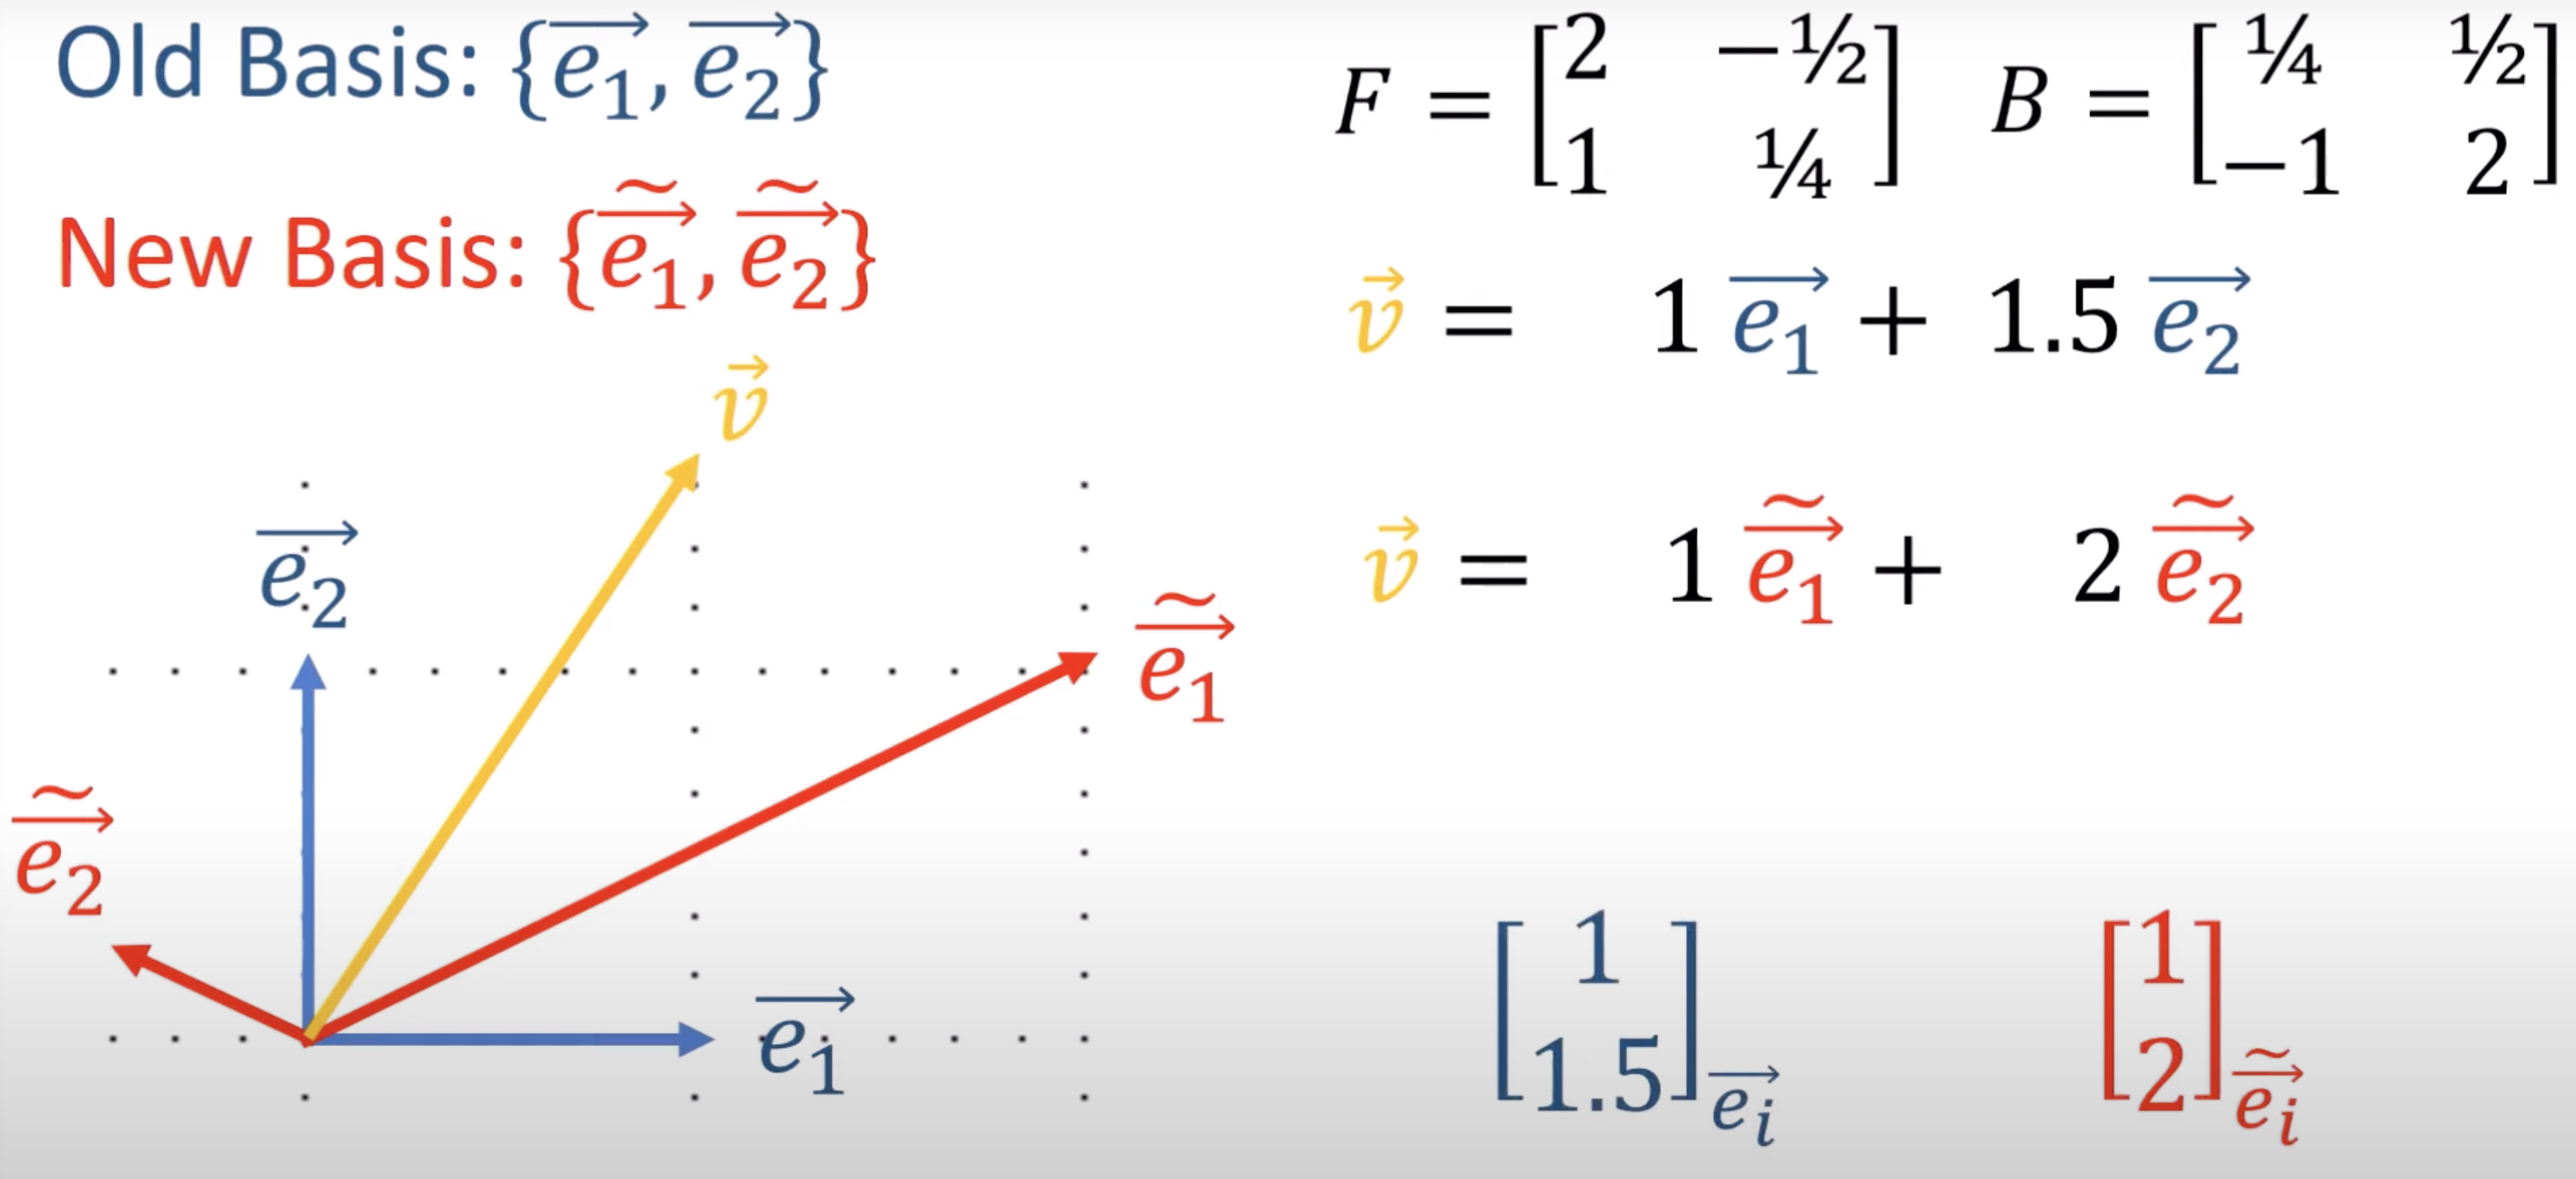
\includegraphics[width=0.7\textwidth]{vector_example_eigenchris}
  \caption{vector example in old and new system}
  \label{fig:vector_example_old_new_base}
\end{figure}

Vectors are formed by linear combinations of their basis vectors with the coordinates as
scaling coefficients of the corresponding basis vectors:
\begin{subequations}
  \begin{align}
    \label{eq:vector_def_old}
    \hdv & =  \sum\limits_i \hdvc{i} \hdbv{i} = \hdvc{i} \hdbvc{i}
    \quad\text{(summation convention)} \\
    \label{eq:vector_def_new}
    \hdv & = \sum\limits_i \hdtvc{i} \hdbtv{i} = \hdtvc{i} \hdbtvc{i}
    \quad\text{(summation convention)}
  \end{align}
\end{subequations}

Inserting the backward transformation (\ref{eq:backward_trafo}) in
(\ref{eq:vector_def_old}) and re-arranging the sums by exchanging the indices, we can get
the transformation rule of the vector components by comparing with
(\ref{eq:vector_def_new}). This yields the transformation rule for the vector components:
\begin{equation}
  \label{eq:vector_trafo_to_new}
  \begin{array}{rcl}
    \hdv & = & \hdvc{i} \hdbvc{i}
    = \hdvc{i} B^{j~}_{~i} \hdbtvc{j}
    = \hdvc{j} B^{i~}_{~j} \hdbtvc{i} \\
    \hdv & = & \hdtvc{i} \hdbtvc{i}
    \\ \noalign{\vskip10pt}
    \Rightarrow \hdtvc{i} & = & B^{i~}_{~j} \hdvc{j}
  \end{array}
\end{equation}

By inserting the forward transformation (\ref{eq:forward_trafo}) in
(\ref{eq:vector_def_new}) and re-arranging the sums, we can get the transformation rule of
the vector components by comparing with (\ref{eq:vector_def_old}). This yields the
transformation rule for the vector components in the other direction:
\begin{equation}
  \label{eq:vector_trafo_to_old}
  \begin{array}{rcl}
    \hdv & = & \hdvc{i} \hdbvc{i} \\
    \hdv & = & \hdtvc{i} \hdbtvc{i}
    = \hdtvc{i} F^{j~}_{~i}\hdbvc{j}
    = \hdtvc{j} F^{i~}_{~j}\hdbvc{i}\\
    \noalign{\vskip10pt}
    \Rightarrow \hdvc{i} & = &  F^{i~}_{~j} \hdtvc{j}
  \end{array}
\end{equation}

Summarizing the transformation rules for basis vectors and the respective vector
compontents we get:
\begin{equation}
  \label{eq:vector_trafo_overview}
  \begin{array}{rclrcl}
    \hdbtvc{i} & = &
    F^{j~}_{~i}\hdbvc{j} \qquad\qquad
    \hdtvc{i} & = & B^{i~}_{~j} \hdvc{j} \\
    \hdbvc{i} & = &
    B^{j~}_{~i}\hdbtvc{j} \qquad\qquad
    \hdvc{i} & = &  F^{i~}_{~j} \hdtvc{j}
  \end{array}
\end{equation}

As can be seen, the basis vectors and their componentens transform with different
transformations. This transformation behaviour is called contravariant. It is the reason
that vectors are called contravariant tensors. \\

For transformation basis vectors are applied to the matrix from the left and vector
components are multiplied from the right for a transformation. This can be seen in the
index notation as well by the position of the indices.
\begin{figure}[h]
  \centering
  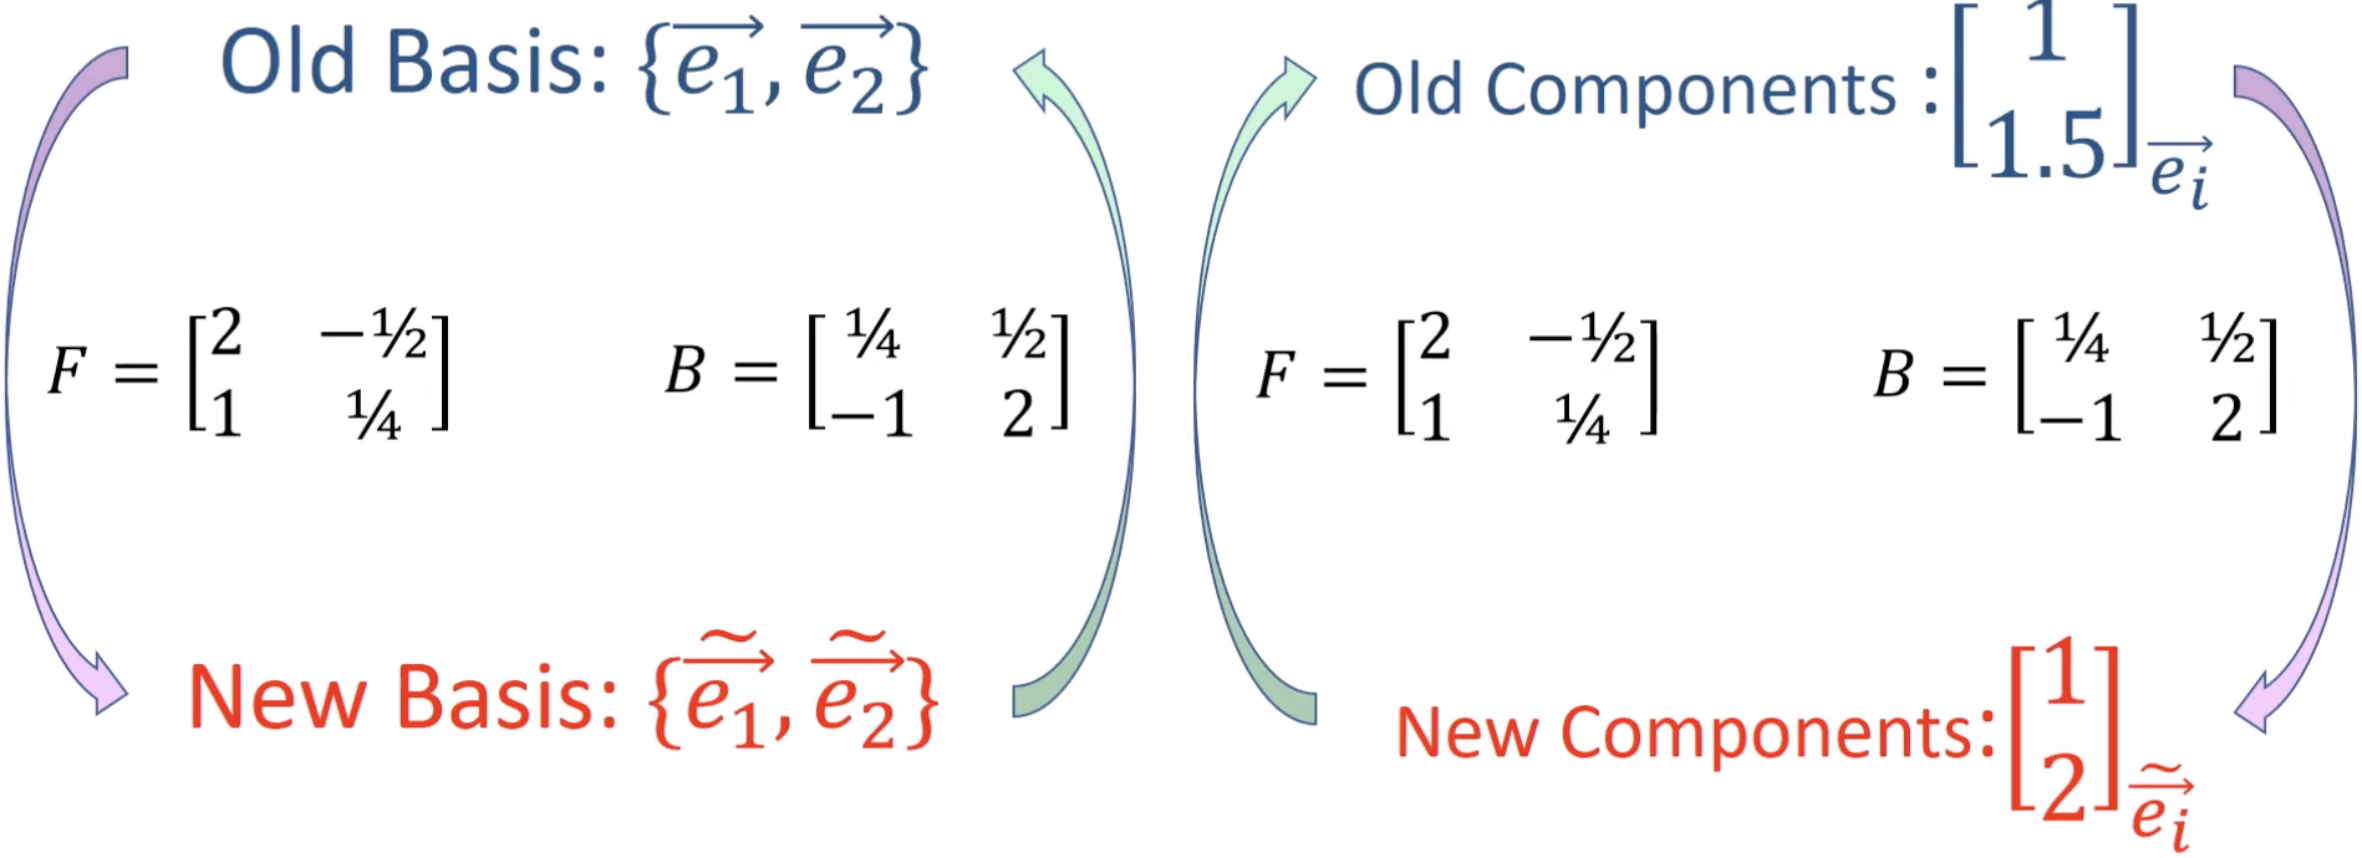
\includegraphics[width=0.65\textwidth]{Summary_transformations_eigenchris}
  \caption{Summary of transformations (example)}
  \label{fig:transformation_summary_example}
\end{figure}

\newpage